% Options for packages loaded elsewhere
\PassOptionsToPackage{unicode}{hyperref}
\PassOptionsToPackage{hyphens}{url}
\PassOptionsToPackage{dvipsnames,svgnames,x11names}{xcolor}
%
\documentclass[
  letterpaper,
  DIV=11,
  numbers=noendperiod]{scrreprt}

\usepackage{amsmath,amssymb}
\usepackage{lmodern}
\usepackage{iftex}
\ifPDFTeX
  \usepackage[T1]{fontenc}
  \usepackage[utf8]{inputenc}
  \usepackage{textcomp} % provide euro and other symbols
\else % if luatex or xetex
  \usepackage{unicode-math}
  \defaultfontfeatures{Scale=MatchLowercase}
  \defaultfontfeatures[\rmfamily]{Ligatures=TeX,Scale=1}
\fi
% Use upquote if available, for straight quotes in verbatim environments
\IfFileExists{upquote.sty}{\usepackage{upquote}}{}
\IfFileExists{microtype.sty}{% use microtype if available
  \usepackage[]{microtype}
  \UseMicrotypeSet[protrusion]{basicmath} % disable protrusion for tt fonts
}{}
\makeatletter
\@ifundefined{KOMAClassName}{% if non-KOMA class
  \IfFileExists{parskip.sty}{%
    \usepackage{parskip}
  }{% else
    \setlength{\parindent}{0pt}
    \setlength{\parskip}{6pt plus 2pt minus 1pt}}
}{% if KOMA class
  \KOMAoptions{parskip=half}}
\makeatother
\usepackage{xcolor}
\setlength{\emergencystretch}{3em} % prevent overfull lines
\setcounter{secnumdepth}{5}
% Make \paragraph and \subparagraph free-standing
\ifx\paragraph\undefined\else
  \let\oldparagraph\paragraph
  \renewcommand{\paragraph}[1]{\oldparagraph{#1}\mbox{}}
\fi
\ifx\subparagraph\undefined\else
  \let\oldsubparagraph\subparagraph
  \renewcommand{\subparagraph}[1]{\oldsubparagraph{#1}\mbox{}}
\fi

\usepackage{color}
\usepackage{fancyvrb}
\newcommand{\VerbBar}{|}
\newcommand{\VERB}{\Verb[commandchars=\\\{\}]}
\DefineVerbatimEnvironment{Highlighting}{Verbatim}{commandchars=\\\{\}}
% Add ',fontsize=\small' for more characters per line
\usepackage{framed}
\definecolor{shadecolor}{RGB}{241,243,245}
\newenvironment{Shaded}{\begin{snugshade}}{\end{snugshade}}
\newcommand{\AlertTok}[1]{\textcolor[rgb]{0.68,0.00,0.00}{#1}}
\newcommand{\AnnotationTok}[1]{\textcolor[rgb]{0.37,0.37,0.37}{#1}}
\newcommand{\AttributeTok}[1]{\textcolor[rgb]{0.40,0.45,0.13}{#1}}
\newcommand{\BaseNTok}[1]{\textcolor[rgb]{0.68,0.00,0.00}{#1}}
\newcommand{\BuiltInTok}[1]{\textcolor[rgb]{0.00,0.23,0.31}{#1}}
\newcommand{\CharTok}[1]{\textcolor[rgb]{0.13,0.47,0.30}{#1}}
\newcommand{\CommentTok}[1]{\textcolor[rgb]{0.37,0.37,0.37}{#1}}
\newcommand{\CommentVarTok}[1]{\textcolor[rgb]{0.37,0.37,0.37}{\textit{#1}}}
\newcommand{\ConstantTok}[1]{\textcolor[rgb]{0.56,0.35,0.01}{#1}}
\newcommand{\ControlFlowTok}[1]{\textcolor[rgb]{0.00,0.23,0.31}{#1}}
\newcommand{\DataTypeTok}[1]{\textcolor[rgb]{0.68,0.00,0.00}{#1}}
\newcommand{\DecValTok}[1]{\textcolor[rgb]{0.68,0.00,0.00}{#1}}
\newcommand{\DocumentationTok}[1]{\textcolor[rgb]{0.37,0.37,0.37}{\textit{#1}}}
\newcommand{\ErrorTok}[1]{\textcolor[rgb]{0.68,0.00,0.00}{#1}}
\newcommand{\ExtensionTok}[1]{\textcolor[rgb]{0.00,0.23,0.31}{#1}}
\newcommand{\FloatTok}[1]{\textcolor[rgb]{0.68,0.00,0.00}{#1}}
\newcommand{\FunctionTok}[1]{\textcolor[rgb]{0.28,0.35,0.67}{#1}}
\newcommand{\ImportTok}[1]{\textcolor[rgb]{0.00,0.46,0.62}{#1}}
\newcommand{\InformationTok}[1]{\textcolor[rgb]{0.37,0.37,0.37}{#1}}
\newcommand{\KeywordTok}[1]{\textcolor[rgb]{0.00,0.23,0.31}{#1}}
\newcommand{\NormalTok}[1]{\textcolor[rgb]{0.00,0.23,0.31}{#1}}
\newcommand{\OperatorTok}[1]{\textcolor[rgb]{0.37,0.37,0.37}{#1}}
\newcommand{\OtherTok}[1]{\textcolor[rgb]{0.00,0.23,0.31}{#1}}
\newcommand{\PreprocessorTok}[1]{\textcolor[rgb]{0.68,0.00,0.00}{#1}}
\newcommand{\RegionMarkerTok}[1]{\textcolor[rgb]{0.00,0.23,0.31}{#1}}
\newcommand{\SpecialCharTok}[1]{\textcolor[rgb]{0.37,0.37,0.37}{#1}}
\newcommand{\SpecialStringTok}[1]{\textcolor[rgb]{0.13,0.47,0.30}{#1}}
\newcommand{\StringTok}[1]{\textcolor[rgb]{0.13,0.47,0.30}{#1}}
\newcommand{\VariableTok}[1]{\textcolor[rgb]{0.07,0.07,0.07}{#1}}
\newcommand{\VerbatimStringTok}[1]{\textcolor[rgb]{0.13,0.47,0.30}{#1}}
\newcommand{\WarningTok}[1]{\textcolor[rgb]{0.37,0.37,0.37}{\textit{#1}}}

\providecommand{\tightlist}{%
  \setlength{\itemsep}{0pt}\setlength{\parskip}{0pt}}\usepackage{longtable,booktabs,array}
\usepackage{calc} % for calculating minipage widths
% Correct order of tables after \paragraph or \subparagraph
\usepackage{etoolbox}
\makeatletter
\patchcmd\longtable{\par}{\if@noskipsec\mbox{}\fi\par}{}{}
\makeatother
% Allow footnotes in longtable head/foot
\IfFileExists{footnotehyper.sty}{\usepackage{footnotehyper}}{\usepackage{footnote}}
\makesavenoteenv{longtable}
\usepackage{graphicx}
\makeatletter
\def\maxwidth{\ifdim\Gin@nat@width>\linewidth\linewidth\else\Gin@nat@width\fi}
\def\maxheight{\ifdim\Gin@nat@height>\textheight\textheight\else\Gin@nat@height\fi}
\makeatother
% Scale images if necessary, so that they will not overflow the page
% margins by default, and it is still possible to overwrite the defaults
% using explicit options in \includegraphics[width, height, ...]{}
\setkeys{Gin}{width=\maxwidth,height=\maxheight,keepaspectratio}
% Set default figure placement to htbp
\makeatletter
\def\fps@figure{htbp}
\makeatother
\newlength{\cslhangindent}
\setlength{\cslhangindent}{1.5em}
\newlength{\csllabelwidth}
\setlength{\csllabelwidth}{3em}
\newlength{\cslentryspacingunit} % times entry-spacing
\setlength{\cslentryspacingunit}{\parskip}
\newenvironment{CSLReferences}[2] % #1 hanging-ident, #2 entry spacing
 {% don't indent paragraphs
  \setlength{\parindent}{0pt}
  % turn on hanging indent if param 1 is 1
  \ifodd #1
  \let\oldpar\par
  \def\par{\hangindent=\cslhangindent\oldpar}
  \fi
  % set entry spacing
  \setlength{\parskip}{#2\cslentryspacingunit}
 }%
 {}
\usepackage{calc}
\newcommand{\CSLBlock}[1]{#1\hfill\break}
\newcommand{\CSLLeftMargin}[1]{\parbox[t]{\csllabelwidth}{#1}}
\newcommand{\CSLRightInline}[1]{\parbox[t]{\linewidth - \csllabelwidth}{#1}\break}
\newcommand{\CSLIndent}[1]{\hspace{\cslhangindent}#1}

\KOMAoption{captions}{tableheading}
\makeatletter
\makeatother
\makeatletter
\@ifpackageloaded{bookmark}{}{\usepackage{bookmark}}
\makeatother
\makeatletter
\@ifpackageloaded{caption}{}{\usepackage{caption}}
\AtBeginDocument{%
\ifdefined\contentsname
  \renewcommand*\contentsname{Table of contents}
\else
  \newcommand\contentsname{Table of contents}
\fi
\ifdefined\listfigurename
  \renewcommand*\listfigurename{List of Figures}
\else
  \newcommand\listfigurename{List of Figures}
\fi
\ifdefined\listtablename
  \renewcommand*\listtablename{List of Tables}
\else
  \newcommand\listtablename{List of Tables}
\fi
\ifdefined\figurename
  \renewcommand*\figurename{Figure}
\else
  \newcommand\figurename{Figure}
\fi
\ifdefined\tablename
  \renewcommand*\tablename{Table}
\else
  \newcommand\tablename{Table}
\fi
}
\@ifpackageloaded{float}{}{\usepackage{float}}
\floatstyle{ruled}
\@ifundefined{c@chapter}{\newfloat{codelisting}{h}{lop}}{\newfloat{codelisting}{h}{lop}[chapter]}
\floatname{codelisting}{Listing}
\newcommand*\listoflistings{\listof{codelisting}{List of Listings}}
\makeatother
\makeatletter
\@ifpackageloaded{caption}{}{\usepackage{caption}}
\@ifpackageloaded{subcaption}{}{\usepackage{subcaption}}
\makeatother
\makeatletter
\@ifpackageloaded{tcolorbox}{}{\usepackage[many]{tcolorbox}}
\makeatother
\makeatletter
\@ifundefined{shadecolor}{\definecolor{shadecolor}{rgb}{.97, .97, .97}}
\makeatother
\makeatletter
\makeatother
\ifLuaTeX
  \usepackage{selnolig}  % disable illegal ligatures
\fi
\IfFileExists{bookmark.sty}{\usepackage{bookmark}}{\usepackage{hyperref}}
\IfFileExists{xurl.sty}{\usepackage{xurl}}{} % add URL line breaks if available
\urlstyle{same} % disable monospaced font for URLs
\hypersetup{
  pdftitle={Resping Data with tidyr},
  pdfauthor={Saul Diaz Infante Velasco},
  colorlinks=true,
  linkcolor={blue},
  filecolor={Maroon},
  citecolor={Blue},
  urlcolor={Blue},
  pdfcreator={LaTeX via pandoc}}

\title{Resping Data with tidyr}
\author{Saul Diaz Infante Velasco}
\date{3/16/23}

\begin{document}
\maketitle
\ifdefined\Shaded\renewenvironment{Shaded}{\begin{tcolorbox}[breakable, borderline west={3pt}{0pt}{shadecolor}, enhanced, interior hidden, frame hidden, sharp corners, boxrule=0pt]}{\end{tcolorbox}}\fi

\renewcommand*\contentsname{Table of contents}
{
\hypersetup{linkcolor=}
\setcounter{tocdepth}{2}
\tableofcontents
}
\bookmarksetup{startatroot}

\hypertarget{preface}{%
\chapter*{Preface}\label{preface}}
\addcontentsline{toc}{chapter}{Preface}

\markboth{Preface}{Preface}

Preface for this part

\bookmarksetup{startatroot}

\hypertarget{introduction}{%
\chapter*{Introduction}\label{introduction}}
\addcontentsline{toc}{chapter}{Introduction}

\markboth{Introduction}{Introduction}

Data in the wild can be scary---when confronted with a complicated and
messy dataset you may find yourself wondering, where do I even start?
The \texttt{tidyr} package allows you to wrangle such beasts into nice
and tidy datasets. Inaccessible values stored in column names will be
put into rows, JSON files will become data frames, and missing values
will never go missing again. You'll practice these techniques on a wide
range of messy datasets, learning along the way how many dogs the Soviet
Union sent into space and what bird is most popular in New Zealand. With
the tidyr package in your tidyverse toolkit, you'll be able to transform
almost any dataset in a tidy format which will pay-off during the rest
of your analysis.

\bookmarksetup{startatroot}

\hypertarget{tidy-data}{%
\chapter{Tidy Data}\label{tidy-data}}

You'll be introduced to the concept of tidy data which is central to
this course. In the first two lessons, you'll jump straight into the
action by separating messy character columns into tidy variables and
observations ready for analysis. In the final lesson, you'll learn how
to overwrite and remove missing values.

\hypertarget{multiple-variables-per-column}{%
\section{Multiple variables per
column}\label{multiple-variables-per-column}}

Being a busy person, you don't want to spend too much time on Netflix,
so you decide to crunch some numbers on TV show and movie durations
before deciding what to watch. You've managed to obtain a dataset named
\texttt{netflix\_df}, but its \texttt{duration} column has an issue. It
contains strings with both a value and unit of duration (\texttt{"min"}
or \texttt{"Season"}).

You'll tidy this dataset so that each variable gets its own column.

As will always be the case in this course, load the tidyr package.

\hypertarget{instructions-100-xp}{%
\subsection*{\texorpdfstring{Instructions
\texttt{100\ XP}}{Instructions 100 XP}}\label{instructions-100-xp}}
\addcontentsline{toc}{subsection}{Instructions \texttt{100\ XP}}

\begin{itemize}
\tightlist
\item
  Inspect \texttt{netflix\_df} by typing its name directly in the R
  console and hitting Enter to see what string separates the value from
  the unit in the \texttt{duration} column.
\item
  Separate the \texttt{duration} column over two variables named
  \texttt{value} and \texttt{unit}. Pass the string separating the
  number from the unit to the \texttt{sep} argument.
\end{itemize}

\textbf{ex\_001.R}

\begin{Shaded}
\begin{Highlighting}[]
\NormalTok{netflix\_df }\SpecialCharTok{\%\textgreater{}\%} 
  \CommentTok{\# Split the duration column into value and unit columns}
  \FunctionTok{separate}\NormalTok{(duration, }\AttributeTok{into =}\FunctionTok{c}\NormalTok{(}\StringTok{"value"}\NormalTok{,}\StringTok{"unit"}\NormalTok{),}\AttributeTok{sep =} \StringTok{" "}\NormalTok{, }\AttributeTok{convert =} \ConstantTok{TRUE}\NormalTok{)}
\end{Highlighting}
\end{Shaded}

\hypertarget{international-phone-numbers}{%
\section{International phone
numbers}\label{international-phone-numbers}}

You work for a multinational company that uses auto-dialer software to
contact its customers. When new customers subscribe online they are
asked for a phone number but they often forget to add the country code
needed for international calls. You were asked to fix this issue in the
database. You've been given a data frame with national numbers and
country codes named \texttt{phone\_nr\_df}. Now you want to combine the
country\_code and \texttt{national\_number} columns to create valid
international numbers.

\hypertarget{instructions-100-xp-1}{%
\subsection*{\texorpdfstring{Instructions
\texttt{100\ XP}}{Instructions 100 XP}}\label{instructions-100-xp-1}}
\addcontentsline{toc}{subsection}{Instructions \texttt{100\ XP}}

Use the \texttt{unite()} function to create a new
\texttt{international\_number} column, using an empty string as the
separator.

\textbf{ex\_002.R}

\begin{Shaded}
\begin{Highlighting}[]
\NormalTok{phone\_nr\_df }\SpecialCharTok{\%\textgreater{}\%}
  \CommentTok{\# Unite the country\_code and national\_number columns}
  \FunctionTok{unite}\NormalTok{(}
    \StringTok{"international\_number"}\NormalTok{,}
\NormalTok{    country\_code,}
\NormalTok{    national\_number,}
    \AttributeTok{sep=}\StringTok{""}
\NormalTok{  )}
\end{Highlighting}
\end{Shaded}

\hypertarget{extracting-observations-from-values}{%
\section{Extracting observations from
values}\label{extracting-observations-from-values}}

Extracting observations from values You're given a sample of the Netflix
dataset containing TV shows and their casts called \texttt{tvshow\_df}.
You want to learn which six actors have the most appearances.

However, the dataset only has one row per TV show, and multiple actors
are listed in the cast column.

Transform the data so that for each TV show, every actor has a row. The
number of appearances will be calculated for you.

Load dplyr package.

\hypertarget{instructions-100-xp-2}{%
\subsection*{\texorpdfstring{Instructions
\texttt{100\ XP}}{Instructions 100 XP}}\label{instructions-100-xp-2}}
\addcontentsline{toc}{subsection}{Instructions \texttt{100\ XP}}

\begin{itemize}
\tightlist
\item
  Use \texttt{separate\_rows()} on the cast column, using the
  appropriate separator for the sep argument.
\item
  Use the \texttt{head()} function to keep just the top six.
\end{itemize}

\textbf{ex\_003.R}

\begin{Shaded}
\begin{Highlighting}[]
\NormalTok{tvshow\_df }\SpecialCharTok{\%\textgreater{}\%} 
  \CommentTok{\# Separate the actors in the cast column over multiple rows}
  \FunctionTok{separate\_rows}\NormalTok{(cast, }\AttributeTok{sep=}\StringTok{", "}\NormalTok{) }\SpecialCharTok{\%\textgreater{}\%} 
  \FunctionTok{rename}\NormalTok{(}\AttributeTok{actor =}\NormalTok{ cast) }\SpecialCharTok{\%\textgreater{}\%} 
  \FunctionTok{count}\NormalTok{(actor, }\AttributeTok{sort =} \ConstantTok{TRUE}\NormalTok{) }\SpecialCharTok{\%\textgreater{}\%} 
  \FunctionTok{head}\NormalTok{()}
\end{Highlighting}
\end{Shaded}

\hypertarget{separating-into-columns-and-rows}{%
\section{Separating into columns and
rows}\label{separating-into-columns-and-rows}}

Remember the drink ingredients data from the video? You've been given a
similar version (\texttt{drink\_df}) that also includes quantities and
units. Now you want to create an overview of how much of each ingredient
you should buy to make these drinks.

Load \texttt{dplyr}.

\hypertarget{instructions-100-xp-3}{%
\subsection*{\texorpdfstring{Instructions
\texttt{100\ XP}}{Instructions 100 XP}}\label{instructions-100-xp-3}}
\addcontentsline{toc}{subsection}{Instructions \texttt{100\ XP}}

\begin{itemize}
\tightlist
\item
  Inspect \texttt{drink\_df} in the console to find the right separator
  in the \texttt{ingredients} column.
\item
  Separate the \texttt{ingredients} column so that for each drink each
  ingredient gets a row. -Inspect the output of the previous step to
  find the separator that splits the ingredients column into three
  columns: \texttt{ingredient}, \texttt{quantity}, and \texttt{unit}.
  -Make sure to convert data types to numeric when possible.
\end{itemize}

\textbf{ex\_004.R}

\begin{Shaded}
\begin{Highlighting}[]
\NormalTok{drink\_df }\SpecialCharTok{\%\textgreater{}\%} 
  \CommentTok{\# Separate the ingredients over rows}
  \FunctionTok{separate\_rows}\NormalTok{(ingredients, }\AttributeTok{sep =} \StringTok{"; "}\NormalTok{) }\SpecialCharTok{\%\textgreater{}\%} 
  \CommentTok{\# Separate ingredients into three columns}
  \FunctionTok{separate}\NormalTok{(}
\NormalTok{    ingredients, }
    \AttributeTok{into =} \FunctionTok{c}\NormalTok{(}\StringTok{"ingredient"}\NormalTok{, }\StringTok{"quantity"}\NormalTok{, }\StringTok{"unit"}\NormalTok{), }
    \AttributeTok{sep =} \StringTok{" "}\NormalTok{, }
    \AttributeTok{convert =} \ConstantTok{TRUE}
\NormalTok{  ) }\SpecialCharTok{\%\textgreater{}\%} 
  \CommentTok{\# Group by ingredient and unit}
  \FunctionTok{group\_by}\NormalTok{(ingredient, unit) }\SpecialCharTok{\%\textgreater{}\%} 
  \CommentTok{\# Calculate the total quantity of each ingredient}
  \FunctionTok{summarize}\NormalTok{(}\AttributeTok{quantity =} \FunctionTok{sum}\NormalTok{(quantity))}
\end{Highlighting}
\end{Shaded}

\hypertarget{and-the-oscar-tfor-best-director-goet-to-..}{%
\section{\texorpdfstring{And the Oscar tfor best director goet to ..
}{And the Oscar tfor best director goet to .. }}\label{and-the-oscar-tfor-best-director-goet-to-..}}

You're working on a sample of the Netflix dataset pre-loaded as
\texttt{director\_df}. This time, the data frame contains just the
directors and movie titles. Your goal is to identify the directors who
created the most movies. Since the \texttt{director} column contains
multiple names, you'll first separate its values over multiple rows and
then count the directors.

Since you don't want movies without directors polluting your overview,
you'll apply the \texttt{drop\_na()} function.

Load dplyr package.

\hypertarget{instructions-100-xp-4}{%
\subsection*{\texorpdfstring{Instructions
\texttt{100\ XP}}{Instructions 100 XP}}\label{instructions-100-xp-4}}
\addcontentsline{toc}{subsection}{Instructions \texttt{100\ XP}}

\begin{itemize}
\tightlist
\item
  Inspect \texttt{director\_df} in the console to see what string
  separates directors in the \texttt{director} column.
\item
  Spread the values in the \texttt{director} column over separate rows.
\item
  Count the number of times each director appears in the data. Make sure
  to sort the output.
\item
  Drop rows containing NA values in the director column.
\end{itemize}

\textbf{ex\_005.R}

\begin{Shaded}
\begin{Highlighting}[]
\NormalTok{director\_df }\SpecialCharTok{\%\textgreater{}\%} 
  \CommentTok{\# Spread the director column over separate rows}
  \FunctionTok{separate\_rows}\NormalTok{(}
\NormalTok{    director,}
    \AttributeTok{sep =} \StringTok{", "}
\NormalTok{  )}

\NormalTok{director\_df }\SpecialCharTok{\%\textgreater{}\%} 
  \CommentTok{\# Spread the director column over separate rows}
  \FunctionTok{separate\_rows}\NormalTok{(director, }\AttributeTok{sep =} \StringTok{", "}\NormalTok{) }\SpecialCharTok{\%\textgreater{}\%} 
  \CommentTok{\# Count the number of movies per director}
  \FunctionTok{count}\NormalTok{(director)}

\NormalTok{director\_df }\SpecialCharTok{\%\textgreater{}\%} 
  \CommentTok{\# Spread the director column over separate rows}
  \FunctionTok{separate\_rows}\NormalTok{(director, }\AttributeTok{sep =} \StringTok{", "}\NormalTok{) }\SpecialCharTok{\%\textgreater{}\%} 
  \CommentTok{\# Count the number of movies per director}
  \FunctionTok{count}\NormalTok{(director, }\AttributeTok{sort=}\ConstantTok{TRUE}\NormalTok{) }

\NormalTok{director\_df }\SpecialCharTok{\%\textgreater{}\%} 
  \CommentTok{\# Drop rows with NA values in the director column}
  \FunctionTok{drop\_na}\NormalTok{(director) }\SpecialCharTok{\%\textgreater{}\%} 
  \CommentTok{\# Spread the director column over separate rows}
  \FunctionTok{separate\_rows}\NormalTok{(director, }\AttributeTok{sep =} \StringTok{", "}\NormalTok{) }\SpecialCharTok{\%\textgreater{}\%} 
  \CommentTok{\# Count the number of movies per director}
  \FunctionTok{count}\NormalTok{(director, }\AttributeTok{sort =} \ConstantTok{TRUE}\NormalTok{)}
\end{Highlighting}
\end{Shaded}

\hypertarget{imputing-sales-data}{%
\section{Imputing sales data}\label{imputing-sales-data}}

You've been asked to create a report that allows management to compare
sales figures per quarter for two years. The problem is that the dataset
(\texttt{sales\_df}) contains missing values. You'll need to impute the
values in the year column so that you can visualize the data.

Load \texttt{ggplot2}.

\hypertarget{instructions-100-xp-5}{%
\subsection*{\texorpdfstring{Instructions
\texttt{100\ XP}}{Instructions 100 XP}}\label{instructions-100-xp-5}}
\addcontentsline{toc}{subsection}{Instructions \texttt{100\ XP}}

\begin{itemize}
\tightlist
\item
  Inspect \texttt{sales\_df} in the console, pay attention to the year
  column.
\item
  Use the \texttt{fill()} function to impute the year column in the
  correct direction.
\item
  Create a line \texttt{plot} where each year has a different color.
\end{itemize}

\textbf{ex\_006.R}

\begin{Shaded}
\begin{Highlighting}[]
\NormalTok{sales\_df }\SpecialCharTok{\%\textgreater{}\%} 
  \CommentTok{\# Impute the year column}
  \FunctionTok{fill}\NormalTok{(year, }\AttributeTok{.direction =} \StringTok{"up"}\NormalTok{) }\SpecialCharTok{\%\textgreater{}\%}
  \CommentTok{\# Create a line plot with sales per quarter colored by year.}
  \FunctionTok{ggplot}\NormalTok{(}
    \FunctionTok{aes}\NormalTok{(}
      \AttributeTok{x =}\NormalTok{ quarter,}
      \AttributeTok{y =}\NormalTok{ sales,}
      \AttributeTok{color =}\NormalTok{ year,}
      \AttributeTok{group =}\NormalTok{ year}
\NormalTok{    )}
\NormalTok{  ) }\SpecialCharTok{+}
  \FunctionTok{geom\_line}\NormalTok{()}
\end{Highlighting}
\end{Shaded}

\hypertarget{nuclear-bombs-per-continent}{%
\section{Nuclear bombs per
continent}\label{nuclear-bombs-per-continent}}

Since WWII, a number of nations have been detonating nuclear bombs for
military research. A tally of bombs detonated per nation has been
calculated from the Nuclear Explosion DataBase (NEDB) and provided as
\texttt{nuke\_df}. You are interested in finding out how many bombs have
been detonated by nations grouped per continent. To achieve this goal,
\texttt{nuke\_df} will be joined to \texttt{country\_to\_continent\_df}
which is a mapping of nation to continent. You will need to overwrite
missing values with zeros so that you can create a nice plot.

Load \texttt{dplyr} and \texttt{ggplot2}.

\begin{description}
\tightlist
\item[Side note 1:]
Bombs detonated by the Soviet Union were attributed to the Russian
Federation.
\item[Side note 2:]
The Russian Federation is solely mapped to Europe for simplicity.
\end{description}

\hypertarget{instructions-100-xp-6}{%
\subsection*{\texorpdfstring{Instructions
\texttt{100\ XP}}{Instructions 100 XP}}\label{instructions-100-xp-6}}
\addcontentsline{toc}{subsection}{Instructions \texttt{100\ XP}}

\begin{itemize}
\tightlist
\item
  Inspect \texttt{nuke\_df} and \texttt{country\_to\_continent\_df} in
  the console.
\item
  Replace the missing values in the \texttt{n\_bombs} columns with
  \texttt{0L}. Adding the L sets the data type to integer.
\item
  Group the dataset by \texttt{continent} and aggregate the data by
  summing the number of bombs.
\item
  Plot the summed number of bombs detonated by nations from each
  continent.
\end{itemize}

\textbf{ex\_007.R}

\begin{Shaded}
\begin{Highlighting}[]
\NormalTok{  country\_to\_continent\_df }\SpecialCharTok{\%\textgreater{}\%} 
  \FunctionTok{left\_join}\NormalTok{(nuke\_df, }\AttributeTok{by =} \StringTok{"country\_code"}\NormalTok{) }\SpecialCharTok{\%\textgreater{}\%}  
  \CommentTok{\# Impute the missing values in the n\_bombs column with 0L}
  \FunctionTok{replace\_na}\NormalTok{(}\FunctionTok{list}\NormalTok{(}\AttributeTok{n\_bombs =}\NormalTok{ 0L)) }\SpecialCharTok{\%\textgreater{}\%} 
  \CommentTok{\# Group the dataset by continent}
  \FunctionTok{group\_by}\NormalTok{(continent) }\SpecialCharTok{\%\textgreater{}\%} 
  \CommentTok{\# Sum the number of bombs per continent}
  \FunctionTok{summarize}\NormalTok{(}\AttributeTok{n\_bombs\_continent =} \FunctionTok{sum}\NormalTok{(n\_bombs)) }\SpecialCharTok{\%\textgreater{}\%} 
  \CommentTok{\# Plot the number of bombs per continent}
  \FunctionTok{ggplot}\NormalTok{(}\FunctionTok{aes}\NormalTok{(}\AttributeTok{x =}\NormalTok{ continent, }\AttributeTok{y =}\NormalTok{ n\_bombs\_continent)) }\SpecialCharTok{+}
  \FunctionTok{geom\_col}\NormalTok{()}
\end{Highlighting}
\end{Shaded}

\bookmarksetup{startatroot}

\hypertarget{from-wide-to-long-and-back}{%
\chapter{From Wide to Long and Back}\label{from-wide-to-long-and-back}}

This chapter is all about pivoting data from a wide to long format and
back again using the \texttt{pivot\_longer()} and
\texttt{pivot\_wider()} functions. You'll need these functions when
variables are hidden in messy column names or when variables are stored
in rows instead of columns. You'll learn about space dogs, nuclear
bombs, and planet temperatures along the way.

\hypertarget{nuclear-bombs-per-country}{%
\section{Nuclear bombs per country}\label{nuclear-bombs-per-country}}

You've been given a version of the Nuclear Explosion DataBase (NEDB)
where country names are specified in the column headers (nuke\_df). You
want to visualize how many nukes were detonated per year per country.
You'll need to pivot the data and replace NA values first.

The ggplot2 package is needed.

\hypertarget{instructions-100-xp-7}{%
\subsection*{\texorpdfstring{Instructions
\texttt{100\ XP}}{Instructions 100 XP}}\label{instructions-100-xp-7}}
\addcontentsline{toc}{subsection}{Instructions \texttt{100\ XP}}

Pivot all columns except for year to a longer format.

\textbf{ex\_008.R}

\begin{Shaded}
\begin{Highlighting}[]
\NormalTok{nuke\_df }\SpecialCharTok{\%\textgreater{}\%} 
  \CommentTok{\# Pivot the data to a longer format}
  \FunctionTok{pivot\_longer}\NormalTok{(}\SpecialCharTok{{-}}\StringTok{"year"}\NormalTok{)}

\NormalTok{nuke\_df }\SpecialCharTok{\%\textgreater{}\%} 
  \CommentTok{\# Pivot the data to a longer format}
  \FunctionTok{pivot\_longer}\NormalTok{(}
    \SpecialCharTok{{-}}\NormalTok{year, }
    \CommentTok{\# Overwrite the names of the two new columns}
    \AttributeTok{names\_to =} \StringTok{"country"}\NormalTok{, }
    \AttributeTok{values\_to =} \StringTok{"n\_bombs"}
\NormalTok{  )}

\NormalTok{nuke\_df }\SpecialCharTok{\%\textgreater{}\%} 
  \CommentTok{\# Pivot the data to a longer format}
  \FunctionTok{pivot\_longer}\NormalTok{(}
    \SpecialCharTok{{-}}\NormalTok{year, }
    \CommentTok{\# Overwrite the names of the two new columns}
    \AttributeTok{names\_to =} \StringTok{"country"}\NormalTok{, }
    \AttributeTok{values\_to =} \StringTok{"n\_bombs"}
\NormalTok{  ) }\SpecialCharTok{\%\textgreater{}\%}
  \CommentTok{\# Replace NA values for n\_bombs with 0L}
  \FunctionTok{replace\_na}\NormalTok{(}\FunctionTok{list}\NormalTok{(}\AttributeTok{n\_bombs =}\NormalTok{ 0L))}

\NormalTok{  nuke\_df }\SpecialCharTok{\%\textgreater{}\%} 
  \CommentTok{\# Pivot the data to a longer format}
  \FunctionTok{pivot\_longer}\NormalTok{(}
    \SpecialCharTok{{-}}\NormalTok{year, }
    \CommentTok{\# Overwrite the names of the two new columns}
    \AttributeTok{names\_to =} \StringTok{"country"}\NormalTok{, }
    \AttributeTok{values\_to =} \StringTok{"n\_bombs"}
\NormalTok{  ) }\SpecialCharTok{\%\textgreater{}\%} 
  \CommentTok{\# Replace NA values for n\_bombs with 0L}
  \FunctionTok{replace\_na}\NormalTok{(}\FunctionTok{list}\NormalTok{(}\AttributeTok{n\_bombs =}\NormalTok{ 0L)) }\SpecialCharTok{\%\textgreater{}\%} 
  \CommentTok{\# Plot the number of bombs per country over time}
  \FunctionTok{ggplot}\NormalTok{(}\FunctionTok{aes}\NormalTok{(}\AttributeTok{x=}\NormalTok{year, }\AttributeTok{y=}\NormalTok{n\_bombs, }\AttributeTok{group=}\NormalTok{country, }\AttributeTok{color=}\NormalTok{country)) }\SpecialCharTok{+}
    \FunctionTok{geom\_line}\NormalTok{()}

\end{Highlighting}
\end{Shaded}

\hypertarget{who-obesity-per-country}{%
\section{WHO obesity per country}\label{who-obesity-per-country}}

According to the World Health Organization (WHO), worldwide obesity has
nearly tripled since 1975. You're interested in the severity of this
global health issue per country and whether males and females are
affected differently. You'll use the WHO's obesity data (obesity\_df) to
investigate this issue. The data holds the percentage of females, males,
and both sexes combined that are considered obese (BMI \textgreater{}
30) per country.

You want to create a scatterplot where, per nation, you can see the
obesity data colored differently for females and males. This implies
that sex should become a variable with its own column.

Load the ggplot2 package.

\hypertarget{instructions-100-xp-8}{%
\subsection*{\texorpdfstring{Instructions
\texttt{100\ XP}}{Instructions 100 XP}}\label{instructions-100-xp-8}}
\addcontentsline{toc}{subsection}{Instructions \texttt{100\ XP}}

\begin{itemize}
\tightlist
\item
  Pivot the male and female columns. The old column names should go in
  the sex column, the original values should go in the pct\_obese
  column.
\end{itemize}

\textbf{ex\_009.R}

\begin{Shaded}
\begin{Highlighting}[]
\NormalTok{obesity\_df }\SpecialCharTok{\%\textgreater{}\%} 
  \CommentTok{\# Pivot the male and female columns}
  \FunctionTok{pivot\_longer}\NormalTok{(}
    \FunctionTok{c}\NormalTok{(}\StringTok{"male"}\NormalTok{, }\StringTok{"female"}\NormalTok{),}
    \AttributeTok{names\_to =} \StringTok{"sex"}\NormalTok{,}
    \AttributeTok{values\_to =} \StringTok{"pct\_obese"}
\NormalTok{  )}
\NormalTok{obesity\_df }\SpecialCharTok{\%\textgreater{}\%} 
  \CommentTok{\# Pivot the male and female columns}
  \FunctionTok{pivot\_longer}\NormalTok{(}\FunctionTok{c}\NormalTok{(male, female),}
               \AttributeTok{names\_to =} \StringTok{"sex"}\NormalTok{,}
               \AttributeTok{values\_to =} \StringTok{"pct\_obese"}\NormalTok{) }\SpecialCharTok{\%\textgreater{}\%} 
  \CommentTok{\# Create a scatter plot with pct\_obese per country colored by sex}
  \FunctionTok{ggplot}\NormalTok{(}\FunctionTok{aes}\NormalTok{(}\AttributeTok{x =}\NormalTok{ country, }\AttributeTok{color =}\NormalTok{ sex,}
             \AttributeTok{y =}\NormalTok{ forcats}\SpecialCharTok{::}\FunctionTok{fct\_reorder}\NormalTok{(country, both\_sexes))) }\SpecialCharTok{+}
  \FunctionTok{geom\_point}\NormalTok{() }\SpecialCharTok{+}
  \FunctionTok{scale\_y\_discrete}\NormalTok{(}\AttributeTok{breaks =} \FunctionTok{c}\NormalTok{(}\StringTok{"India"}\NormalTok{, }\StringTok{"Nauru"}\NormalTok{, }\StringTok{"Cuba"}\NormalTok{, }\StringTok{"Brazil"}\NormalTok{,}
                              \StringTok{"Pakistan"}\NormalTok{, }\StringTok{"Gabon"}\NormalTok{, }\StringTok{"Italy"}\NormalTok{, }\StringTok{"Oman"}\NormalTok{,}
                              \StringTok{"China"}\NormalTok{, }\StringTok{"United States of America"}\NormalTok{)) }\SpecialCharTok{+}
  \FunctionTok{labs}\NormalTok{(}\AttributeTok{x =} \StringTok{"\% Obese"}\NormalTok{, }\AttributeTok{y =} \StringTok{"Country"}\NormalTok{)}
\end{Highlighting}
\end{Shaded}

\hypertarget{bond-james-bond}{%
\section{Bond\ldots{} James Bond}\label{bond-james-bond}}

You've been given a James Bond movie dataset (\texttt{bond\_df}) and
want to visualize the number of movies that Bond actors have featured in
per decade. However, the data is in an untidy format with the decade
values captured in the column headers. You'll tidy this dataset to give
each variable its own column.

The ggplot2 package is needed.

\hypertarget{instructions-100-xp-9}{%
\subsection*{\texorpdfstring{Instructions
\texttt{100\ XP}}{Instructions 100 XP}}\label{instructions-100-xp-9}}
\addcontentsline{toc}{subsection}{Instructions \texttt{100\ XP}}

\textbf{ex\_010.R}

\begin{Shaded}
\begin{Highlighting}[]
\NormalTok{bond\_df }\SpecialCharTok{\%\textgreater{}\%} 
  \CommentTok{\# Pivot the data to long format and set the column names}
\FunctionTok{pivot\_longer}\NormalTok{(}
  \FunctionTok{c}\NormalTok{(}
    \StringTok{\textasciigrave{}}\AttributeTok{1960}\StringTok{\textasciigrave{}}\NormalTok{,}
    \StringTok{\textasciigrave{}}\AttributeTok{1970}\StringTok{\textasciigrave{}}\NormalTok{,}
    \StringTok{\textasciigrave{}}\AttributeTok{1980}\StringTok{\textasciigrave{}}\NormalTok{,}
    \StringTok{\textasciigrave{}}\AttributeTok{1990}\StringTok{\textasciigrave{}}\NormalTok{,}
    \StringTok{\textasciigrave{}}\AttributeTok{2000}\StringTok{\textasciigrave{}}\NormalTok{,}
    \StringTok{\textasciigrave{}}\AttributeTok{2010}\StringTok{\textasciigrave{}}\NormalTok{,}
    \StringTok{\textasciigrave{}}\AttributeTok{2020}\StringTok{\textasciigrave{}}
\NormalTok{  ),}
  \AttributeTok{names\_to =} \StringTok{"decade"}\NormalTok{,}
  \AttributeTok{values\_to =} \StringTok{"n\_movies"}
\NormalTok{)}
\NormalTok{bond\_df }\SpecialCharTok{\%\textgreater{}\%} 
  \CommentTok{\# Pivot the data to long format}
  \FunctionTok{pivot\_longer}\NormalTok{(}
    \SpecialCharTok{{-}}\NormalTok{Bond, }
    \CommentTok{\# Overwrite the names of the two newly created columns}
    \AttributeTok{names\_to =} \StringTok{"decade"}\NormalTok{, }
    \AttributeTok{values\_to =} \StringTok{"n\_movies"}\NormalTok{, }
    \CommentTok{\# Drop na values}
    \AttributeTok{values\_drop\_na =} \ConstantTok{TRUE}
\NormalTok{  )}
\NormalTok{  bond\_df }\SpecialCharTok{\%\textgreater{}\%} 
  \CommentTok{\# Pivot the data to long format}
  \FunctionTok{pivot\_longer}\NormalTok{(}
    \SpecialCharTok{{-}}\NormalTok{Bond, }
    \CommentTok{\# Overwrite the names of the two newly created columns}
    \AttributeTok{names\_to =} \StringTok{"decade"}\NormalTok{, }
    \AttributeTok{values\_to =} \StringTok{"n\_movies"}\NormalTok{, }
    \CommentTok{\# Drop na values}
    \AttributeTok{values\_drop\_na =} \ConstantTok{TRUE}\NormalTok{, }
    \CommentTok{\# Transform the decade column data type to integer}
    \AttributeTok{names\_transform =} \FunctionTok{list}\NormalTok{(}\AttributeTok{decade =}\NormalTok{ as.integer)  }
\NormalTok{  ) }\SpecialCharTok{\%\textgreater{}\%} 
  \FunctionTok{ggplot}\NormalTok{(}\FunctionTok{aes}\NormalTok{(}\AttributeTok{x =}\NormalTok{ decade }\SpecialCharTok{+} \DecValTok{5}\NormalTok{, }\AttributeTok{y =}\NormalTok{ n\_movies, }\AttributeTok{fill =}\NormalTok{ Bond))}\SpecialCharTok{+}
  \FunctionTok{geom\_col}\NormalTok{()}
\end{Highlighting}
\end{Shaded}

\hypertarget{new-zealands-bird-of-the-year}{%
\section{New-Zealand's bird of the
year}\label{new-zealands-bird-of-the-year}}

Every year New Zealanders vote en masse to decide which species gets the
bird of the year trophy. The contest is organized by the Forest \& Bird
agency which allows each person to give points to up to five birds
(first pick gets 5 points, second 4, \ldots). Your job is to decide this
year's winner from the messy dataset that's been pre-loaded for you as
bird\_df.

The dplyr package is needed. \#\#\# Instructions \texttt{100\ XP}
\{.unnumbered\}

\textbf{ex\_011.R}

\begin{Shaded}
\begin{Highlighting}[]
\NormalTok{bird\_df }\SpecialCharTok{\%\textgreater{}\%}
  \CommentTok{\# Pivot the data to create a two column data frame}
  \FunctionTok{pivot\_longer}\NormalTok{(}
    \FunctionTok{c}\NormalTok{(points\_5, points\_4, points\_3, points\_2, points\_1),}
    \AttributeTok{names\_to =} \StringTok{"points"}\NormalTok{,}
    \AttributeTok{names\_prefix =} \StringTok{"points\_"}\NormalTok{,}
    \AttributeTok{names\_transform =} \FunctionTok{list}\NormalTok{(}\AttributeTok{points =}\NormalTok{ as.integer),}
    \AttributeTok{values\_to =} \StringTok{"species"}\NormalTok{,}
    \AttributeTok{values\_drop\_na =} \ConstantTok{TRUE}
\NormalTok{  )}
\NormalTok{bird\_df }\SpecialCharTok{\%\textgreater{}\%}
  \CommentTok{\# Pivot the data to create a 2 column data frame}
  \FunctionTok{pivot\_longer}\NormalTok{(}
    \FunctionTok{starts\_with}\NormalTok{(}\StringTok{"points\_"}\NormalTok{),}
    \AttributeTok{names\_to =} \StringTok{"points"}\NormalTok{,}
    \AttributeTok{names\_prefix =} \StringTok{"points\_"}\NormalTok{,}
    \AttributeTok{names\_transform =} \FunctionTok{list}\NormalTok{(}\AttributeTok{points =}\NormalTok{ as.integer),}
    \AttributeTok{values\_to =} \StringTok{"species"}\NormalTok{,}
    \AttributeTok{values\_drop\_na =} \ConstantTok{TRUE}
\NormalTok{  ) }\SpecialCharTok{\%\textgreater{}\%}
  \FunctionTok{group\_by}\NormalTok{(species) }\SpecialCharTok{\%\textgreater{}\%} 
  \FunctionTok{summarize}\NormalTok{(}\AttributeTok{total\_points=}\FunctionTok{sum}\NormalTok{(points)) }\SpecialCharTok{\%\textgreater{}\%} 
  \FunctionTok{slice\_max}\NormalTok{(total\_points, }\AttributeTok{n =} \DecValTok{5}\NormalTok{)}
\end{Highlighting}
\end{Shaded}

\hypertarget{big-tech-stock-prices}{%
\section{Big tech stock prices}\label{big-tech-stock-prices}}

You're an analyst at an investment firm and want to visualize the weekly
closing prices of five big tech firms' stocks. However, the dataset
you've been handed (\texttt{stock\_df}) is messy and has the year and
week variables stored in the column headers. You'll pivot this data into
a tidy format, extract the variables from the headers, and create a line
plot.

Load the ggplot2 package. \#\#\# Instructions \texttt{100\ XP}
\{.unnumbered\} - Pivot stock\_df so that the integer columns year and
week are created from the column names and the original values are moved
to the price column. Use the \texttt{names\_sep} argument to separate
the column names.

\textbf{ex\_012.R}

\begin{Shaded}
\begin{Highlighting}[]
\NormalTok{stock\_df }\SpecialCharTok{\%\textgreater{}\%} 
  \CommentTok{\# Pivot the data to create 3 new columns: year, week, price}
\FunctionTok{pivot\_longer}\NormalTok{(}
  \SpecialCharTok{{-}}\NormalTok{company,}
  \AttributeTok{names\_to =} \FunctionTok{c}\NormalTok{(}\StringTok{"year"}\NormalTok{, }\StringTok{"week"}\NormalTok{),}
  \AttributeTok{names\_transform =} \FunctionTok{list}\NormalTok{(}\AttributeTok{year=}\NormalTok{as.integer, }\AttributeTok{week=}\NormalTok{as.integer),}
  \AttributeTok{values\_to =} \StringTok{"price"}\NormalTok{, }
  \AttributeTok{names\_sep =} \StringTok{"\_week"}
\NormalTok{)}

\NormalTok{stock\_df }\SpecialCharTok{\%\textgreater{}\%} 
  \CommentTok{\# Pivot the data to create 3 new columns: year, week, price}
  \FunctionTok{pivot\_longer}\NormalTok{(}
    \SpecialCharTok{{-}}\NormalTok{company,}
    \AttributeTok{names\_to =} \FunctionTok{c}\NormalTok{(}\StringTok{"year"}\NormalTok{, }\StringTok{"week"}\NormalTok{),}
    \AttributeTok{values\_to =} \StringTok{"price"}\NormalTok{,}
    \AttributeTok{names\_sep =} \StringTok{"\_week"}\NormalTok{,}
    \AttributeTok{names\_transform =} \FunctionTok{list}\NormalTok{(}
      \AttributeTok{year =}\NormalTok{ as.integer,}
      \AttributeTok{week =}\NormalTok{ as.integer)}
\NormalTok{  ) }\SpecialCharTok{\%\textgreater{}\%}
  \CommentTok{\# Create a line plot with price per week, color by company}
  \FunctionTok{ggplot}\NormalTok{(}\FunctionTok{aes}\NormalTok{(}\AttributeTok{x=}\NormalTok{week, }\AttributeTok{y=}\NormalTok{price, }\FunctionTok{group}\NormalTok{(company), }\AttributeTok{color=}\NormalTok{company)) }\SpecialCharTok{+}
  \FunctionTok{geom\_line}\NormalTok{() }\SpecialCharTok{+}
  \FunctionTok{facet\_grid}\NormalTok{(. }\SpecialCharTok{\textasciitilde{}}\NormalTok{ year)}
\end{Highlighting}
\end{Shaded}

\hypertarget{soviet-space-dogs-the-dogs-perspective}{%
\section{Soviet space dogs, the dogs
perspective}\label{soviet-space-dogs-the-dogs-perspective}}

You'll be working on an pre-processed sample of the USSR space dogs
database compiled by Duncan Geere and pre-loaded for you as
\texttt{space\_dogs\_df}. Each of the 42 rows in this dataset represents
a test rocket launch which had one or two very brave dogs on board.

Your goal is to reshape this dataset so that for each launch, each dog
has a row.

The challenge is that in the column headers (\texttt{name\_1},
\texttt{name\_2}, \texttt{gender\_1}, and \texttt{gender\_2}), the part
before the \texttt{\_} separator can point to two different variables
(name and gender), while the second part always points to the dog ID
(1st or 2nd dog).

\hypertarget{instructions-100-xp-10}{%
\subsection*{\texorpdfstring{Instructions
\texttt{100\ XP}}{Instructions 100 XP}}\label{instructions-100-xp-10}}
\addcontentsline{toc}{subsection}{Instructions \texttt{100\ XP}}

\begin{itemize}
\tightlist
\item
  As the first argument to pivot\_longer(), pass the columns to pivot
  (\texttt{name\_1}, \texttt{name\_2}, \texttt{gender\_1}, and
  \texttt{gender\_2}).
\item
  Complete the names\_to argument so that the first part of the column
  headers are reused.
\item
  Make sure NA values are dropped since not all rockets had two dogs.
\end{itemize}

\textbf{ex\_013.R}

\begin{Shaded}
\begin{Highlighting}[]
\NormalTok{space\_dogs\_df }\SpecialCharTok{\%\textgreater{}\%} 
  \FunctionTok{pivot\_longer}\NormalTok{(}
    \CommentTok{\# Add the columns to pivot}
    \FunctionTok{c}\NormalTok{(}
      \StringTok{"name\_1"}\NormalTok{,}
      \StringTok{"name\_2"}\NormalTok{,}
      \StringTok{"gender\_1"}\NormalTok{,}
      \StringTok{"gender\_2"}
\NormalTok{    ),}
    \AttributeTok{names\_sep =} \StringTok{"\_"}\NormalTok{,}
    \CommentTok{\# Complete the names\_to argument to re{-}use the first part of the column headers}
    \AttributeTok{names\_to =} \FunctionTok{c}\NormalTok{(}\StringTok{".value"}\NormalTok{,  }\StringTok{"dog\_id"}\NormalTok{),}
    \CommentTok{\# Make sure NA values are dropped}
    \AttributeTok{values\_drop\_na =} \ConstantTok{TRUE}
\NormalTok{  )}
\end{Highlighting}
\end{Shaded}

\hypertarget{who-obesity-vs.-life-expectancy}{%
\section{WHO obesity vs.~life
expectancy}\label{who-obesity-vs.-life-expectancy}}

You've been given a sample of WHO data (\texttt{who\_df}) with obesity
percentages and life expectancy data per country, year, and sex. You
want to visually inspect the correlation between obesity and life
expectancy.

However, the data is very messy with four variables hidden in the column
names. Each column name is made up of three parts separated by
underscores: Values for the year, followed by those for \texttt{sex},
and then values for either \texttt{pct.obese} or \texttt{life.exp}.
Since the third part of the column name string holds two variables
you'll need to use the special ``\texttt{.value}'' value in the
\texttt{names\_to} argument.

You'll pivot the data into a tidy format and create the
\texttt{scatterplot}.

Load the \texttt{ggplot2} package.

\hypertarget{instructions-100-xp-11}{%
\subsection*{\texorpdfstring{Instructions
\texttt{100\ XP}}{Instructions 100 XP}}\label{instructions-100-xp-11}}
\addcontentsline{toc}{subsection}{Instructions \texttt{100\ XP}}

\textbf{ex\_014.R}

\begin{Shaded}
\begin{Highlighting}[]
\NormalTok{who\_df }\SpecialCharTok{\%\textgreater{}\%} 
  \CommentTok{\# Put each variable in its own column}
  \FunctionTok{pivot\_longer}\NormalTok{(}
    \SpecialCharTok{{-}}\NormalTok{country,}
    \AttributeTok{names\_to =} \FunctionTok{c}\NormalTok{(}\StringTok{"year"}\NormalTok{, }\StringTok{"sex"}\NormalTok{, }\StringTok{".value"}\NormalTok{),}
    \AttributeTok{names\_sep =} \StringTok{"\_"}\NormalTok{, }
    \AttributeTok{names\_transform =} \FunctionTok{list}\NormalTok{(}\StringTok{"year"} \OtherTok{=}\NormalTok{ as.integer)}
\NormalTok{  ) }\SpecialCharTok{\%\textgreater{}\%}
  \CommentTok{\# Create a plot with life expectancy over obesity}
  \FunctionTok{ggplot}\NormalTok{(}
    \FunctionTok{aes}\NormalTok{(}
      \AttributeTok{x =}\NormalTok{ pct.obese,}
      \AttributeTok{y =}\NormalTok{ life.exp,}
      \AttributeTok{color=}\NormalTok{sex}
\NormalTok{    )}
\NormalTok{  ) }\SpecialCharTok{+}
  \FunctionTok{geom\_point}\NormalTok{()}
\end{Highlighting}
\end{Shaded}

\hypertarget{unconting-ovservations}{%
\section{Unconting ovservations}\label{unconting-ovservations}}

You've found the job of your dreams providing technical support for a
dog breed beauty contest. The jury members want a spreadsheet with the
breed and id of each participating dog so that they can add the scores
later on. You've only been given the number of participants per dog
breed (\texttt{dog\_df}) so you decide to use your tidyr skills to
create the desired result.

\hypertarget{instructions-100-xp-12}{%
\subsection*{\texorpdfstring{Instructions
\texttt{100\ XP}}{Instructions 100 XP}}\label{instructions-100-xp-12}}
\addcontentsline{toc}{subsection}{Instructions \texttt{100\ XP}}

\begin{itemize}
\tightlist
\item
  Inspect the data in the console.
\item
  Uncount the data so that per breed, each dog gets a row and an ID. The
  ID should go in the \texttt{dog\_id} column.
\end{itemize}

\textbf{ex\_015.R}

\begin{Shaded}
\begin{Highlighting}[]
\NormalTok{dog\_df }\SpecialCharTok{\%\textgreater{}\%} 
  \CommentTok{\# Create one row for each participant and add the id}
  \FunctionTok{uncount}\NormalTok{(n\_participants, }\AttributeTok{.id =} \StringTok{"dog\_id"}\NormalTok{)}
\end{Highlighting}
\end{Shaded}

\hypertarget{soviet-space-dogs-the-flight-perspective}{%
\section{Soviet space dogs, the flight
perspective}\label{soviet-space-dogs-the-flight-perspective}}

Remember the USSR space dogs dataset\footnote{Compiled by
  \href{https://airtable.com/universe/expG3z2CFykG1dZsp/soviet-space-dogs}{Duncan
  Geere}.}? You changed it to a long format so that for every dog in
every rocket launch, there was a row. Suppose you're given this tidy
dataset and are asked to answer the question, ``In what percentage of
flights were both dogs of the same gender?''

You'll reshape and investigate space\_dogs\_df to find the answer.

The dplyr package has been pre-loaded for you.

\hypertarget{instructions-100-xp-13}{%
\subsection*{\texorpdfstring{Instructions
\texttt{100\ XP}}{Instructions 100 XP}}\label{instructions-100-xp-13}}
\addcontentsline{toc}{subsection}{Instructions \texttt{100\ XP}}

\textbf{ex\_016.R}

\begin{Shaded}
\begin{Highlighting}[]
\NormalTok{space\_dogs\_df }\SpecialCharTok{\%\textgreater{}\%} 
  \CommentTok{\# Pivot the data to a wider format}
  \FunctionTok{pivot\_wider}\NormalTok{(}
    \AttributeTok{names\_from =}\NormalTok{ dog\_id,}
    \AttributeTok{values\_from =}\NormalTok{ gender,}
    \AttributeTok{names\_prefix =} \StringTok{"gender\_"}
\NormalTok{  ) }\SpecialCharTok{\%\textgreater{}\%} 
  \CommentTok{\# Drop rows with NA values}
  \FunctionTok{drop\_na}\NormalTok{() }\SpecialCharTok{\%\textgreater{}\%} 
  \CommentTok{\# Create a Boolean column on whether both dogs have the same gender}
  \FunctionTok{mutate}\NormalTok{(}
    \AttributeTok{same\_gender=} \FunctionTok{ifelse}\NormalTok{(gender\_1}\SpecialCharTok{==}\NormalTok{gender\_2,}
    \ConstantTok{TRUE}\NormalTok{,}
    \ConstantTok{FALSE}
\NormalTok{    )}
\NormalTok{  ) }\SpecialCharTok{\%\textgreater{}\%} 
  \FunctionTok{summarize}\NormalTok{(}\AttributeTok{pct\_same\_gender =} \FunctionTok{mean}\NormalTok{(same\_gender))}
\end{Highlighting}
\end{Shaded}

\hypertarget{planet-temperature-distance-to-the-sun}{%
\section{Planet temperature \& distance to the
Sun}\label{planet-temperature-distance-to-the-sun}}

The intensity of light radiated by a light source follows an inverse
square relationship with the distance it has traveled.
\url{https://en.wikipedia.org/wiki/Inverse-square_law} You wonder if you
could observe this trend in the temperature of the planets in our Solar
System given their distance to the Sun. You'll use the
\texttt{planet\_df} dataset from the
\href{https://devstronomy.com/\#/datasets}{devstronomy} project to
investigate this.

\hypertarget{instructions-100-xp-14}{%
\subsection*{\texorpdfstring{Instructions
\texttt{100\ XP}}{Instructions 100 XP}}\label{instructions-100-xp-14}}
\addcontentsline{toc}{subsection}{Instructions \texttt{100\ XP}}

\begin{itemize}
\tightlist
\item
  Use the \texttt{pivot\_wider()} function to extract column names from
  the \texttt{metric} column and values from the \texttt{value} column.
\end{itemize}

\textbf{ex\_017.R}

\begin{Shaded}
\begin{Highlighting}[]

\NormalTok{planet\_df }\SpecialCharTok{\%\textgreater{}\%} 
  \CommentTok{\# Give each planet variable its own column}
  \FunctionTok{pivot\_wider}\NormalTok{(}
    \AttributeTok{names\_from =}\NormalTok{ metric,}
    \AttributeTok{values\_from =}\NormalTok{ value}
\NormalTok{  )}

\NormalTok{  planet\_df }\SpecialCharTok{\%\textgreater{}\%} 
  \CommentTok{\# Give each planet variable its own column}
  \FunctionTok{pivot\_wider}\NormalTok{(}
    \AttributeTok{names\_from =}\NormalTok{ metric,}
    \AttributeTok{values\_from =}\NormalTok{ value}
\NormalTok{  )}
\end{Highlighting}
\end{Shaded}

\hypertarget{transporting-plantet-data}{%
\section{Transporting plantet data}\label{transporting-plantet-data}}

You're again working on a planet dataset derived from the
\href{https://devstronomy.com/\#/datasets}{devstronomy} project. This
time, you're interested in the correlation between the diameter of a
planet and the number of moons circling it.

However, the dataset (\texttt{planet\_df}) has a row for each variable
and a column for each planet (\texttt{observation}). You'll transpose
this data in two steps and then create a plot to inspect the
correlation.

Load ggplot2 package.

\hypertarget{instructions-100-xp-15}{%
\subsection*{\texorpdfstring{Instructions
\texttt{100\ XP}}{Instructions 100 XP}}\label{instructions-100-xp-15}}
\addcontentsline{toc}{subsection}{Instructions \texttt{100\ XP}}

\begin{itemize}
\tightlist
\item
  Pivot the data so that planet names are put in a column named
  \texttt{planet}.
\item
  Pivot the data so that each variable in the \texttt{metric} column
  gets its own column.
\item
  Use the \texttt{ggplot()} function to create a plot with the
  \texttt{number\_of\_moons} over \texttt{diameter}.
\end{itemize}

\textbf{ex\_018.R}

\begin{Shaded}
\begin{Highlighting}[]

\NormalTok{planet\_df }\SpecialCharTok{\%\textgreater{}\%}
  \CommentTok{\# Pivot all columns except metric to long format}
  \FunctionTok{pivot\_longer}\NormalTok{(}
    \SpecialCharTok{{-}}\NormalTok{metric, }
    \AttributeTok{names\_to =} \StringTok{"planet"}
\NormalTok{  )}

\NormalTok{planet\_df }\SpecialCharTok{\%\textgreater{}\%}
  \CommentTok{\# Pivot all columns except metric to long format}
  \FunctionTok{pivot\_longer}\NormalTok{(}\SpecialCharTok{{-}}\NormalTok{metric, }\AttributeTok{names\_to =} \StringTok{"planet"}\NormalTok{) }\SpecialCharTok{\%\textgreater{}\%} 
  \CommentTok{\# Put each metric in its own column}
  \FunctionTok{pivot\_wider}\NormalTok{(}\AttributeTok{names\_from =}\NormalTok{ metric, }\AttributeTok{values\_from =}\NormalTok{ value) }\SpecialCharTok{\%\textgreater{}\%} 
  \CommentTok{\# Plot the number of moons vs. planet diameter}
  \FunctionTok{ggplot}\NormalTok{(}\FunctionTok{aes}\NormalTok{(}\AttributeTok{x=}\NormalTok{diameter, }\AttributeTok{y=}\NormalTok{number\_of\_moons)) }\SpecialCharTok{+}
  \FunctionTok{geom\_point}\NormalTok{(}\FunctionTok{aes}\NormalTok{(}\AttributeTok{size =}\NormalTok{ diameter)) }\SpecialCharTok{+}
  \FunctionTok{geom\_text}\NormalTok{(}\FunctionTok{aes}\NormalTok{(}\AttributeTok{label =}\NormalTok{ planet), }\AttributeTok{vjust =} \SpecialCharTok{{-}}\DecValTok{1}\NormalTok{) }\SpecialCharTok{+}
  \FunctionTok{labs}\NormalTok{(}\AttributeTok{x =} \StringTok{"Diameter (km)"}\NormalTok{, }\AttributeTok{y =} \StringTok{"Number of moons"}\NormalTok{) }\SpecialCharTok{+}
  \FunctionTok{theme}\NormalTok{(}\AttributeTok{legend.position =} \StringTok{"none"}\NormalTok{)}

\end{Highlighting}
\end{Shaded}

\bookmarksetup{startatroot}

\hypertarget{expanding-data}{%
\chapter{Expanding Data}\label{expanding-data}}

Values can often be missing in your data, and sometimes entire
observations are absent too. In this chapter, you'll learn how to
complete your dataset with these missing observations. You'll add
observations with zero values to counted data, expand time series to a
full sequence of intervals, and more!

\hypertarget{letters-of-the-genetic-code}{%
\section{Letters of the genetic
code}\label{letters-of-the-genetic-code}}

The basic building blocks of \textbf{RNA} are four molecules described
by a single letter each: adenine (\textbf{A}), cytosine (\textbf{C}),
guanine (\textbf{G}), and uracil (\textbf{U}). The information carried
by an RNA strand can be represented as a long sequence of these four
letters. To read this code, one has to divide this chain into sequences
of three letters each (e.g.** GCU, ACG**, \ldots). These three letter
sequences are known as codons. The concept is illustrated in the image
below.

\begin{figure}

{\centering 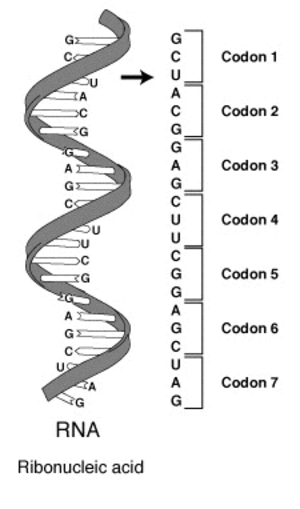
\includegraphics{./rna.png}

}

\caption{Helix rna model}

\end{figure}

\hypertarget{instructions-100-xp-16}{%
\subsection*{\texorpdfstring{Instructions
\texttt{100\ XP}}{Instructions 100 XP}}\label{instructions-100-xp-16}}
\addcontentsline{toc}{subsection}{Instructions \texttt{100\ XP}}

\begin{itemize}
\tightlist
\item
  Create a tibble with three columns called \texttt{letter1},
  \texttt{letter2}, and \texttt{letter3} that holds all possible
  combinations of the vector letters using \texttt{expand\_grid()}.
\item
  Use the \texttt{unite()} function from chapter one to merge these
  three columns into a single column named codon. Use an empty string as
  the separator.
\end{itemize}

\textbf{ex\_019.R}

\begin{Shaded}
\begin{Highlighting}[]
\NormalTok{letters }\OtherTok{\textless{}{-}} \FunctionTok{c}\NormalTok{(}\StringTok{"A"}\NormalTok{, }\StringTok{"C"}\NormalTok{, }\StringTok{"G"}\NormalTok{, }\StringTok{"U"}\NormalTok{)}
\CommentTok{\# Create a tibble with all possible 3 way combinations}
\NormalTok{codon\_df }\OtherTok{\textless{}{-}} \FunctionTok{expand\_grid}\NormalTok{(}
    \AttributeTok{leter1 =}\NormalTok{ letters,}
    \AttributeTok{leter2 =}\NormalTok{ letters,}
    \AttributeTok{leter3 =}\NormalTok{ letters}
\NormalTok{)}
\NormalTok{codon\_df}

\NormalTok{letters }\OtherTok{\textless{}{-}} \FunctionTok{c}\NormalTok{(}\StringTok{"A"}\NormalTok{, }\StringTok{"C"}\NormalTok{, }\StringTok{"G"}\NormalTok{, }\StringTok{"U"}\NormalTok{)}
\CommentTok{\# Create a tibble with all possible 3 way combinations}
\NormalTok{codon\_df }\OtherTok{\textless{}{-}} \FunctionTok{expand\_grid}\NormalTok{(}
  \AttributeTok{letter1 =}\NormalTok{ letters,}
  \AttributeTok{letter2 =}\NormalTok{ letters,}
  \AttributeTok{letter3 =}\NormalTok{ letters}
\NormalTok{)}
\CommentTok{\#}
\NormalTok{codon\_df }\SpecialCharTok{\%\textgreater{}\%} 
  \CommentTok{\# Unite these three columns into a "codon" column}
  \FunctionTok{unite}\NormalTok{(}\StringTok{"codon"}\NormalTok{,  }\FunctionTok{c}\NormalTok{(letter1, letter2, letter3),}
    \AttributeTok{sep =} \StringTok{\textquotesingle{}\textquotesingle{}}
\NormalTok{  )}
\end{Highlighting}
\end{Shaded}

\hypertarget{when-did-humans-replace-dogs-in-space}{%
\section{When did humans replace dogs in
space}\label{when-did-humans-replace-dogs-in-space}}

You already know that in the early days of spaceflight, the USSR was
testing rockets with dogs. You now wonder when exactly humans started
replacing dogs on space flight missions. You've been given a dataset
\texttt{space\_df} with the number of both dogs (compiled by Duncan
Geere) and humans in space per year from 1951 till 1970 (collected from
Wikipedia).

Your goal is to create a plot that shows you the number of individuals
sent into space per species. Before you can create this plot, you'll
first have to introduce zero values for missing combinations of
\texttt{year} and \texttt{species}.

Load dplyr and ggplot2 packages.

\hypertarget{instructions-100-xp-17}{%
\subsection*{\texorpdfstring{Instructions
\texttt{100\ XP}}{Instructions 100 XP}}\label{instructions-100-xp-17}}
\addcontentsline{toc}{subsection}{Instructions \texttt{100\ XP}}

\begin{itemize}
\tightlist
\item
  Create \texttt{full\_df}, a tibble with all unique combinations of the
  variables year (from 1951 to 1970) and \texttt{species}
  (\texttt{"Human"} and \texttt{"Dog"}).
\item
  Perform a \texttt{right\_join()} between \texttt{space\_df} and
  \texttt{full\_df} on the \texttt{year} and species columns.
\item
  Use the ggplot() function to create a line plot of n\_in\_space over
  year, colored by species.
\item
  Use the replace\_na() function to overwrite NA values in the
  n\_in\_space column with zeros.
\end{itemize}

\textbf{ex\_020.R}

\begin{Shaded}
\begin{Highlighting}[]
\CommentTok{\# Create a tibble with all combinations of years and species}
\NormalTok{full\_df }\OtherTok{\textless{}{-}} \FunctionTok{expand\_grid}\NormalTok{(}
  \AttributeTok{year =} \DecValTok{1951}\SpecialCharTok{:}\DecValTok{1970}\NormalTok{, }
  \AttributeTok{species =} \FunctionTok{c}\NormalTok{(}\StringTok{"Human"}\NormalTok{, }\StringTok{"Dog"}\NormalTok{)}
\NormalTok{)}

\NormalTok{space\_df }\SpecialCharTok{\%\textgreater{}\%} 
  \CommentTok{\# Join with full\_df so that missing values are introduced}
  \FunctionTok{right\_join}\NormalTok{(full\_df, }\AttributeTok{by =} \FunctionTok{c}\NormalTok{(}\StringTok{"year"}\NormalTok{, }\StringTok{"species"}\NormalTok{)) }\SpecialCharTok{\%\textgreater{}\%} 
  \CommentTok{\# Create a line plot with n\_in\_space over year, color by species}
  \FunctionTok{ggplot}\NormalTok{(}
    \FunctionTok{aes}\NormalTok{(}
      \AttributeTok{x =}\NormalTok{ n\_in\_space,}
      \AttributeTok{y =}\NormalTok{ year,}
      \AttributeTok{group =}\NormalTok{ species,}
      \AttributeTok{color =}\NormalTok{ species}
\NormalTok{    )}
\NormalTok{  ) }\SpecialCharTok{+}
  \FunctionTok{geom\_line}\NormalTok{()}
\CommentTok{\# Create a tibble with all combinations of years and species}
\NormalTok{full\_df }\OtherTok{\textless{}{-}} \FunctionTok{expand\_grid}\NormalTok{(}
  \AttributeTok{year =} \DecValTok{1951}\SpecialCharTok{:}\DecValTok{1970}\NormalTok{, }
  \AttributeTok{species =} \FunctionTok{c}\NormalTok{(}\StringTok{"Human"}\NormalTok{, }\StringTok{"Dog"}\NormalTok{)}
\NormalTok{)}

\NormalTok{space\_df }\SpecialCharTok{\%\textgreater{}\%} 
  \CommentTok{\# Join with full\_df so that missing values are introduced}
  \FunctionTok{right\_join}\NormalTok{(full\_df, }\AttributeTok{by =} \FunctionTok{c}\NormalTok{(}\StringTok{"year"}\NormalTok{, }\StringTok{"species"}\NormalTok{)) }\SpecialCharTok{\%\textgreater{}\%} 
  \CommentTok{\# Overwrite NA values for n\_in\_space with 0L}
  \FunctionTok{replace\_na}\NormalTok{(}\FunctionTok{list}\NormalTok{(}\AttributeTok{n\_in\_space =}\NormalTok{ 0L)) }\SpecialCharTok{\%\textgreater{}\%} 
  \CommentTok{\# Create a line plot with n\_in\_space over year, color by species}
  \FunctionTok{ggplot}\NormalTok{(}\FunctionTok{aes}\NormalTok{(}\AttributeTok{x =}\NormalTok{ year, }\AttributeTok{y =}\NormalTok{ n\_in\_space, }\AttributeTok{color =}\NormalTok{ species)) }\SpecialCharTok{+}
  \FunctionTok{geom\_line}\NormalTok{()}
\end{Highlighting}
\end{Shaded}

\hypertarget{finding-missing-observations}{%
\section{Finding missing
observations}\label{finding-missing-observations}}

You're an inspector at a nuclear plant and have to validate whether
every reactor has received its daily safety check over the course of a
full year. The safety check logs are in \texttt{reactor\_df}, a data
frame with columns date, reactor, and check.

Two vectors, \texttt{dates} and \texttt{reactors}, with all dates of the
year and reactors at the plant respectively have been created for you.
You'll use the combination of the \texttt{expand\_grid()} and
\texttt{anti\_join()} functions to find dates where particular reactors
were not checked.

Load \texttt{dplyr} package.

\hypertarget{instructions-100-xp-18}{%
\subsection*{\texorpdfstring{Instructions
\texttt{100\ XP}}{Instructions 100 XP}}\label{instructions-100-xp-18}}
\addcontentsline{toc}{subsection}{Instructions \texttt{100\ XP}}

\begin{itemize}
\tightlist
\item
  Use the \texttt{expand\_grid()} function to create a tibble holding
  all combinations of the variables date and reactor. Use the dates and
  reactors vectors created for you.
\item
  Perform an anti-join between f\texttt{ull\_df} and
  \texttt{reactor\_df} on the date and reactor columns.
\end{itemize}

\textbf{ex\_021.R}

\begin{Shaded}
\begin{Highlighting}[]
\CommentTok{\# Create a tibble with all combinations of dates and reactors}
\NormalTok{full\_df }\OtherTok{\textless{}{-}} \FunctionTok{expand\_grid}\NormalTok{(}
  \AttributeTok{date =}\NormalTok{ dates, }
  \AttributeTok{reactor =}\NormalTok{ reactors}
\NormalTok{)}

\CommentTok{\# Find the reactor {-} date combinations not present in reactor\_df}
\NormalTok{full\_df }\SpecialCharTok{\%\textgreater{}\%} 
  \FunctionTok{anti\_join}\NormalTok{(reactor\_df, }\AttributeTok{by=}\FunctionTok{c}\NormalTok{(}\StringTok{"date"}\NormalTok{, }\StringTok{"reactor"}\NormalTok{))}
\end{Highlighting}
\end{Shaded}

\hypertarget{completing-the-solar-system}{%
\section{Completing the Solar
System}\label{completing-the-solar-system}}

You have been given a data frame (\texttt{planet\_df}) from the
\href{https://devstronomy.com/\#/datasets}{devstronomy} project with the
number of moons per planet in our Solar System. However, Mercury and
Venus, the two moonless planets, are absent. You want to expand this
dataset using the \texttt{complete()} function and a vector
\texttt{planets} that contains all eight planet's names.

\hypertarget{instructions-100-xp-19}{%
\subsection*{\texorpdfstring{Instructions
\texttt{100\ XP}}{Instructions 100 XP}}\label{instructions-100-xp-19}}
\addcontentsline{toc}{subsection}{Instructions \texttt{100\ XP}}

\begin{itemize}
\tightlist
\item
  Complete the \texttt{planet} variable using the \texttt{planets}
  vector.
\item
  Replace \texttt{NA} values in the \texttt{n\_moons} variable with
  \texttt{0L} values.
\end{itemize}

\textbf{ex\_022.R}

\begin{Shaded}
\begin{Highlighting}[]
\NormalTok{planets }\OtherTok{=} \FunctionTok{c}\NormalTok{(}
    \StringTok{"Mercury"}\NormalTok{,}
    \StringTok{"Venus"}\NormalTok{,}
    \StringTok{"Earth"}\NormalTok{,}
    \StringTok{"Mars"}\NormalTok{,}
    \StringTok{"Jupiter"}\NormalTok{,}
    \StringTok{"Saturn"}\NormalTok{,}
    \StringTok{"Uranus"}\NormalTok{,}
    \StringTok{"Neptune"}
\NormalTok{)}

\NormalTok{planet\_df }\SpecialCharTok{\%\textgreater{}\%} 
  \FunctionTok{complete}\NormalTok{(}
    \CommentTok{\# Complete the planet variable}
    \AttributeTok{planet =}\NormalTok{  planets,}
    \CommentTok{\# Overwrite NA values for n\_moons with 0L}
    \AttributeTok{fill=} \FunctionTok{list}\NormalTok{(}\AttributeTok{n\_moons =}\NormalTok{ 0L)}
\NormalTok{  )}
\end{Highlighting}
\end{Shaded}

\hypertarget{zero-olymoic-medals}{%
\section{Zero Olymoic medals}\label{zero-olymoic-medals}}

Since 1896, athletes from all over the world have been competing in the
modern Olympic games. You've been given a dataset (\texttt{medal\_df})
with observations for all medals won by athletes from the 10 most
successful countries in Olympic history. You want to create a visual
with the number of medals won per country (\texttt{team}) per
\texttt{year}. However, since not all countries won medals each year,
you'll have to introduce zero values before you can make an accurate
visual.


\includegraphics{./olympic_flag_large.png} Load \texttt{ggplot2} and
\texttt{dplyr}. In step 2 and 3 the \texttt{scale\_color\_brewer()}
function is used to color lines in the plot with a palette that makes it
easier to distinguish the different countries.

\hypertarget{instructions-100-xp-20}{%
\subsection*{\texorpdfstring{Instructions
\texttt{100\ XP}}{Instructions 100 XP}}\label{instructions-100-xp-20}}
\addcontentsline{toc}{subsection}{Instructions \texttt{100\ XP}}

\begin{itemize}
\tightlist
\item
  Count the number of medals won per team and year.
\item
  Use \texttt{ggplot()} to create a line plot with \texttt{n\_medals}
  over \texttt{year}, colored by team.
\item
  Complete the \texttt{team} and \texttt{year} variables, replace
  \texttt{NA} values in the \texttt{n\_medals} column with zeros.
\end{itemize}

\textbf{ex\_023.R}

\begin{Shaded}
\begin{Highlighting}[]
\NormalTok{medal\_df }\SpecialCharTok{\%\textgreater{}\%} 
  \CommentTok{\# Count the medals won per team and year}
  \FunctionTok{count}\NormalTok{(team, year, }\AttributeTok{name =} \StringTok{"n\_medals"}\NormalTok{)}
\NormalTok{medal\_df }\SpecialCharTok{\%\textgreater{}\%} 
  \CommentTok{\# Count the medals won per team and year}
  \FunctionTok{count}\NormalTok{(team, year, }\AttributeTok{name =} \StringTok{"n\_medals"}\NormalTok{) }\SpecialCharTok{\%\textgreater{}\%} 
  \CommentTok{\# Plot n\_medals over year, colored by team}
  \FunctionTok{ggplot}\NormalTok{(}
    \FunctionTok{aes}\NormalTok{(}
      \AttributeTok{x =}\NormalTok{ year,}
      \AttributeTok{y =}\NormalTok{ n\_medals,}
      \AttributeTok{group =}\NormalTok{ team,}
      \AttributeTok{color =}\NormalTok{ team}
\NormalTok{    )}
\NormalTok{  ) }\SpecialCharTok{+}
  \FunctionTok{geom\_line}\NormalTok{() }\SpecialCharTok{+}
  \FunctionTok{scale\_color\_brewer}\NormalTok{(}\AttributeTok{palette =} \StringTok{"Paired"}\NormalTok{)}

\NormalTok{medal\_df }\SpecialCharTok{\%\textgreater{}\%} 
  \CommentTok{\# Count the medals won per team and year}
  \FunctionTok{count}\NormalTok{(team, year, }\AttributeTok{name =} \StringTok{"n\_medals"}\NormalTok{) }\SpecialCharTok{\%\textgreater{}\%} 
  \CommentTok{\# Complete the team and year variables, fill n\_medals with zeros}
  \FunctionTok{complete}\NormalTok{(}
\NormalTok{    team,}
\NormalTok{    year,}
    \AttributeTok{fill =} \FunctionTok{list}\NormalTok{(}\AttributeTok{n\_medals =} \DecValTok{0}\NormalTok{)}
\NormalTok{  ) }\SpecialCharTok{\%\textgreater{}\%} 
  \CommentTok{\# Plot n\_medals over year, colored by team}
  \FunctionTok{ggplot}\NormalTok{(}\FunctionTok{aes}\NormalTok{(}\AttributeTok{x =}\NormalTok{ year, }\AttributeTok{y =}\NormalTok{ n\_medals, }\AttributeTok{color =}\NormalTok{ team)) }\SpecialCharTok{+}
  \FunctionTok{geom\_line}\NormalTok{() }\SpecialCharTok{+}
  \FunctionTok{scale\_color\_brewer}\NormalTok{(}\AttributeTok{palette =} \StringTok{"Paired"}\NormalTok{)}
\end{Highlighting}
\end{Shaded}

\hypertarget{creating-a-sequence-with-full_seq}{%
\section{Creating a sequence with
full\_seq()}\label{creating-a-sequence-with-full_seq}}

The \texttt{full\_seq()} function will look for the minimal and maximal
values inside the vector you pass it and will then generate a full
sequence of numbers with a fixed period in between them. When used
inside the \texttt{complete()} function, \texttt{full\_seq()} is a handy
tool to make sure there are no missing observations in your data. Before
combining these two functions you'll generate a few sequences with
\texttt{full\_seq()} on its own to get the hang of this function.

\hypertarget{instructions-100-xp-21}{%
\subsection*{\texorpdfstring{Instructions
\texttt{100\ XP}}{Instructions 100 XP}}\label{instructions-100-xp-21}}
\addcontentsline{toc}{subsection}{Instructions \texttt{100\ XP}}

\begin{itemize}
\tightlist
\item
  Use \texttt{full\_seq()} to create a sequence with all years from 2020
  till 2030.
\item
  Use full\_seq() to create a sequence with all decades from 1980 till
  2030.
\item
  Use full\_seq() to create a sequence with all dates in 1980 using the
  outer\_dates vector.
\end{itemize}

\textbf{ex\_024.R}

\begin{Shaded}
\begin{Highlighting}[]
\CommentTok{\# Generate all years from 2020 to 2030}
\NormalTok{years }\OtherTok{\textless{}{-}} \FunctionTok{full\_seq}\NormalTok{(}\FunctionTok{c}\NormalTok{(}\DecValTok{2020}\NormalTok{, }\DecValTok{2030}\NormalTok{), }\AttributeTok{period =} \DecValTok{1}\NormalTok{)}
\NormalTok{years}
\CommentTok{\# Generate all decades from 1980 to 2030}
\NormalTok{decades }\OtherTok{\textless{}{-}} \FunctionTok{full\_seq}\NormalTok{(}\FunctionTok{c}\NormalTok{(}\DecValTok{1980}\NormalTok{, }\DecValTok{2030}\NormalTok{), }\AttributeTok{period =} \DecValTok{10}\NormalTok{)}
\NormalTok{decades}

\NormalTok{outer\_dates }\OtherTok{\textless{}{-}} \FunctionTok{c}\NormalTok{(}\FunctionTok{as.Date}\NormalTok{(}\StringTok{"1980{-}01{-}01"}\NormalTok{), }\FunctionTok{as.Date}\NormalTok{(}\StringTok{"1980{-}12{-}31"}\NormalTok{))}
\CommentTok{\# Generate the dates for all days in 1980}
\FunctionTok{full\_seq}\NormalTok{(outer\_dates, }\AttributeTok{period =} \DecValTok{1}\NormalTok{)}
\end{Highlighting}
\end{Shaded}

\hypertarget{olympic-medals-per-continent}{%
\section{Olympic medals per
continent}\label{olympic-medals-per-continent}}

\hypertarget{instructions-100-xp-22}{%
\subsection*{\texorpdfstring{Instructions
\texttt{100\ XP}}{Instructions 100 XP}}\label{instructions-100-xp-22}}
\addcontentsline{toc}{subsection}{Instructions \texttt{100\ XP}}

\textbf{ex\_025.R}

\begin{Shaded}
\begin{Highlighting}[]

\end{Highlighting}
\end{Shaded}

\hypertarget{tracking-a-virus-outbreak}{%
\section{Tracking a virus outbreak}\label{tracking-a-virus-outbreak}}

\hypertarget{instructions-100-xp-23}{%
\subsection*{\texorpdfstring{Instructions
\texttt{100\ XP}}{Instructions 100 XP}}\label{instructions-100-xp-23}}
\addcontentsline{toc}{subsection}{Instructions \texttt{100\ XP}}

\textbf{ex\_026.R}

\begin{Shaded}
\begin{Highlighting}[]

\end{Highlighting}
\end{Shaded}

\hypertarget{counting-office-occupants}{%
\section{Counting office occupants}\label{counting-office-occupants}}

\hypertarget{instructions-100-xp-24}{%
\subsection*{\texorpdfstring{Instructions
\texttt{100\ XP}}{Instructions 100 XP}}\label{instructions-100-xp-24}}
\addcontentsline{toc}{subsection}{Instructions \texttt{100\ XP}}

\textbf{ex\_027.R}

\begin{Shaded}
\begin{Highlighting}[]

\end{Highlighting}
\end{Shaded}

\bookmarksetup{startatroot}

\hypertarget{rectangling-data}{%
\chapter{Rectangling Data}\label{rectangling-data}}

\bookmarksetup{startatroot}

\hypertarget{summary}{%
\chapter{Summary}\label{summary}}

In summary, this book has no content whatsoever.

\bookmarksetup{startatroot}

\hypertarget{references}{%
\chapter*{References}\label{references}}
\addcontentsline{toc}{chapter}{References}

\markboth{References}{References}

\hypertarget{refs}{}
\begin{CSLReferences}{0}{0}
\end{CSLReferences}



\end{document}
